\documentclass[]{scrartcl}

\usepackage{mathtools}
\usepackage{subfigure}
\renewcommand{\familydefault}{\sfdefault}
\usepackage{color}
\usepackage{listings}
\definecolor{pblue}{rgb}{0.13,0.13,1}
\definecolor{pgreen}{rgb}{0,0.5,0}
\definecolor{pred}{rgb}{0.9,0,0}
\definecolor{pgrey}{rgb}{0.46,0.45,0.48}
\setlength{\parindent}{0pt}

\lstset{language=Java,
	showspaces=false,
	showtabs=false,
	breaklines=true,
	showstringspaces=false,
	breakatwhitespace=true,
	commentstyle=\color{pgreen},
	keywordstyle=\color{pblue},
	stringstyle=\color{pred},
	basicstyle=\footnotesize
}

%opening
\title{Intelligent Data Management - Exercise 3}
\author{Christoph Prinz}

\begin{document}

\maketitle

\subsection*{Assignment 1}

\begin{tabular}{c|c|c|c|c||c|c|c}
	Element & $S_1$ & $S_2$ & $S_3$  & $S_4$ & $h_1$ & $h_2$ & $h_3$  \\ 
	\hline\hline
	0 & 0 & 1 & 0 & 1 & 1  & 2 & 2 \\ 
	\hline 
	1 & 0 & 1 & 0 & 0 & 3 & 5  & 1 \\ 
	\hline 
	2 & 1 & 0 & 0 & 1 & 5 & 2 & 0  \\ 
	\hline 
	3 & 0 & 0 & 1 & 0 & 1 & 5 & 5 \\ 
	\hline 
	4 & 0 & 0 & 1 & 1 & 3 & 2 & 4 \\ 
	\hline 
	5 & 1 & 0 & 0 & 0 & 5 & 5 & 3 \\ 
\end{tabular} 

\vspace{1cm}

Minhash-Signature Step 1:\\
\begin{tabular}{c||c|c|c|c}
	& $S_1$ & $S_2$ & $S_3$ &$S_4$  \\ 
	\hline \hline
 $h_1$	& $\infty$ & $\infty$ & $\infty$ & $\infty$ \\ 
	\hline 
$h_2$	& $\infty$ & $\infty$ & $\infty$ & $\infty$ \\ 
	\hline 
$h_3$	& $\infty$ & $\infty$ & $\infty$ & $\infty$ \\ 
\end{tabular}

\vspace{1cm}

Minhash-Signature Step 2:\\
\begin{tabular}{c||c|c|c|c}
			& $S_1$ & $S_2$ & $S_3$ &$S_4$  \\ 
	\hline \hline
	$h_1$	&  $\infty$ & 1 & $\infty$ & 1 \\ 
	\hline 
	$h_2$	&  $\infty$ & 2 & $\infty$ & 2 \\ 
	\hline 
	$h_3$	&  $\infty$ & 2 & $\infty$ & 2 \\ 
\end{tabular} 

\vspace{1cm}

Minhash-Signature Step 3:\\
\begin{tabular}{c||c|c|c|c}
	& $S_1$ & $S_2$ & $S_3$ &$S_4$  \\ 
	\hline \hline
	$h_1$	&  $\infty$ & 1 & $\infty$ & 1 \\ 
	\hline 
	$h_2$	&  $\infty$ & 2 & $\infty$ & 2 \\ 
	\hline 
	$h_3$	&  $\infty$ & 1 & $\infty$ & 2 \\ 
\end{tabular} 

\vspace{1cm}

Minhash-Signature Step 4:\\
\begin{tabular}{c||c|c|c|c}
			& $S_1$ & $S_2$ & $S_3$ &$S_4$  \\ 
	\hline \hline
	$h_1$	&  5 & 1 & $\infty$ & 1 \\ 
	\hline 
	$h_2$	&  2 & 2 & $\infty$ & 2 \\ 
	\hline 
	$h_3$	&  0 & 1 & $\infty$ & 0 \\ 
\end{tabular} 

\vspace{1cm}

Minhash-Signature Step 5:\\
\begin{tabular}{c||c|c|c|c}
	& $S_1$ & $S_2$ & $S_3$ &$S_4$  \\ 
	\hline \hline
	$h_1$	&  5 & 1 & 3 & 1 \\ 
	\hline 
	$h_2$	&  2 & 2 & 2 & 2 \\ 
	\hline 
	$h_3$	&  0 & 1 & 4 & 0 \\ 
\end{tabular} 

\vspace{1cm}

Final Minhash-Signature (After Step 6):\\
\begin{tabular}{c||c|c|c|c}
	& $S_1$ & $S_2$ & $S_3$ &$S_4$  \\ 
	\hline \hline
	$h_1$	&  5 & 1 & 3 & 1 \\ 
	\hline 
	$h_2$	&  2 & 2 & 2 & 2 \\ 
	\hline 
	$h_3$	&  0 & 1 & 4 & 0 \\ 
\end{tabular} 

\vspace{1cm}

Jaccard Similarities formula = $|S \cap T| \div |S \cup T|$ \\

$SIM(S_1, S_2) = SIM(\{2, 5\}, \{0, 1\}) = 0$\\\\
$SIM(S_1, S_3) = SIM(\{2, 5\},\{3, 4\}) = 0$\\\\
$SIM(S_1, S_4) = SIM(\{2, 5\}, \{0, 2, 4\}) = \frac{1}{4}$\\\\
$SIM(S_2, S_3) = SIM(\{0, 1\}, \{3, 4\}) = 0$\\\\
$SIM(S_2, S_4) = SIM(\{0, 1\}, \{0, 2, 4\}) = \frac{1}{4}$\\\\
$SIM(S_3, S_4) = SIM(\{3, 4\}, \{0, 2, 4\}) = \frac{1}{4}$\\\\

\subsection*{Assignment 2}

Plots for s-curve:

\begin{figure}[h]
	\centering
	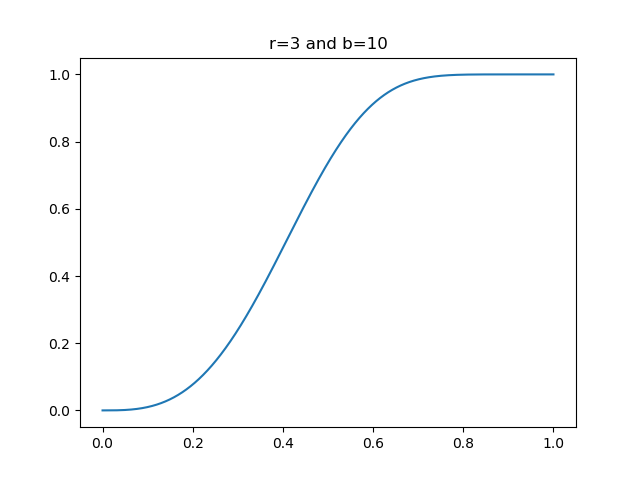
\includegraphics[width=0.5\linewidth]{Exercise4_plots/plot_1}
\end{figure}

\begin{figure}[h]
	\centering
	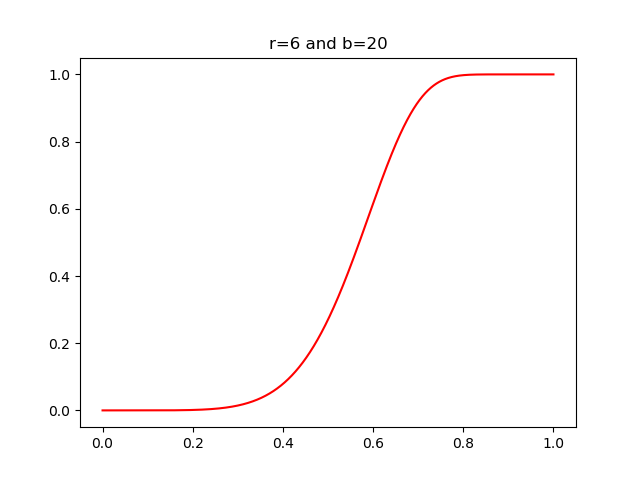
\includegraphics[width=0.5\linewidth]{Exercise4_plots/plot_2}
\end{figure}

\begin{figure}[h]
	\centering
	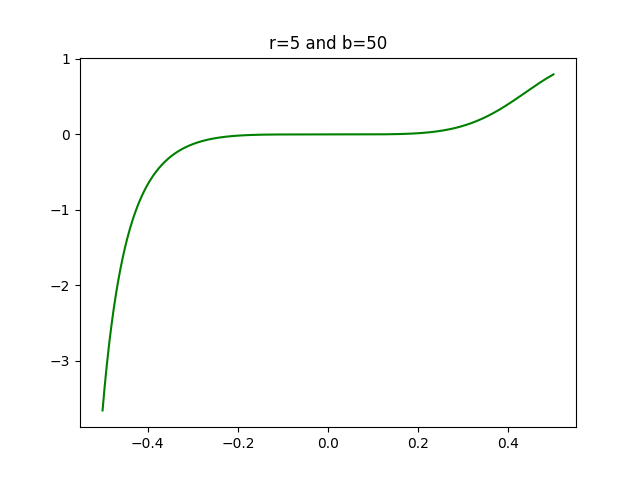
\includegraphics[width=0.5\linewidth]{Exercise4_plots/plot_3}
\end{figure}

%Jaccard Similarities formula = $|S \cap T| \div |S \cup T|$ \\
%
%a) $SIM(\{1, 2, 3, 4\}, \{2, 3, 5, 7\}) = \frac{1}{3}$\\\\
%$SIM(\{1, 2, 3, 4\},\{2, 4, 6\}) = \frac{2}{5}$\\\\
%$SIM(\{2, 3, 5, 7\}, \{2, 4, 6\}) = \frac{1}{6}$\\\\
%
%b) $SIM(\{1, 1, 1, 2\}, \{1, 1, 2, 2, 3\}) = \frac{2}{3}$\\\\
%$SIM(\{1, 1, 1, 2\}, \{1, 2, 3, 4\}) = \frac{1}{2}$\\\\
%$SIM(\{1, 1, 2, 2, 3\}, \{1, 2, 3, 4\}) = \frac{3}{4}$\\
%
%\subsection*{Assignment 2}
%
%a) $\{$The, most, effective$\}$, $\{$most, effective, way$\}$, $\{$effective, way, to$\}$, $\{$way, to, represent$\}$, $\{$to, represent, documents$\}$, $\{$represent, documents, as$\}$, $\{$documents, as, sets$\}$, $\{$as, sets, for$\}$, $\{$sets, for, the$\}$, $\{$for, the, purpose$\}$ \\
%
%
%b) Stopwords are marked as \textit{italic}: "\textit{The} most effective \textit{way} \textit{to} represent documents \textit{as} sets,\textit{ for the} purpose \textit{of} identifying lexically similar documents \textit{is to} construct from \textit{the} document \textit{the set of} short strings that appear within \textit{it}."\\
%
%Resulting Shingles:\\
%
%$\{$The, most, effective$\}$,$\{$way, to, represent$\}$, $\{$to, represent, documents$\}$, $\{$as, sets, for$\}$, $\{$for, the, purpose$\}$, $\{$the, purpose, of$\}$, $\{$of, identifying, lexically$\}$, $\{$is, to, construct$\}$, $\{$to, construct, from$\}$, $\{$the, document, the$\}$, $\{$the, set, of$\}$, $\{$set, of, short $\}$, $\{$of, short, strings$\}$
%
%
% 
%
%%
%%
%%
%%
%%%\subsection*{Exercise a}
%%%
%%%Term $i$ appears in $n_i$ of the $N$ documents \\
%%%
%%%Appears in 40 documents:
%%%$IDF_i = log_2(\frac{N}{n_i}) = log_2(\frac{10000000}{40}) = 18$\\
%%%
%%%Appears in 10000 documents:
%%%$IDF_i = log_2(\frac{N}{n_i}) = log_2(\frac{10000000}{10000}) = 10$ \\
%%%
%%%
%%%\subsection*{Exercise b}
%%%
%%%Given the occurrence of a term $i$ in document $j$ is $f_{ji}$ and $max_k f_{kj}$ the maximum number of occurrences of any term in this document, the term frequency $TF$ is defined as:\\
%%%
%%%$TF_{ij} = \frac{f_{ij}}{max_k f_{kj}}$\\
%%%
%%%Word $w$ appears in 320 documents. In document $d$ the maximum occurence of any word is 15. \\
%%%
%%%a) $w$ appears once:\\
%%%\begin{addmargin}[25pt]{0pt} 
%%%
%%% $TF_{wd} = \frac{1}{15}$\\\\
%%% $IDF_w = * log_2\frac{10000000}{320} = 15$\\\\
%%% $TF.IDF = \frac{1}{15} * 15 = 1$\\\\
%%%
%%%\end{addmargin}
%%%
%%%b) $w$ appears five times: \\
%%%\begin{addmargin}[25pt]{0pt} 
%%%$TF_{wd} = \frac{5}{15} = \frac{1}{3}$\\\\
%%%$IDF_w = * log_2\frac{10000000}{320} = 15$\\\\
%%%$TF.IDF = \frac{1}{3} * 15 = 5$\\\\
%%%\end{addmargin}
%%%
%%%\subsection*{Exercise c}
%%%
%%%The basic rule is, that the possible hash-keys should not have any common factor with B (15 in this example). The population should therefore not be generated with a $c$ of 3 or 5. To achieve an equal distribution of the generated hashs, $c$ should be set to 1.
%%%
%%%\section*{Assignment 2}
%%%
%%%\subsection*{Exercise a}
%%%
%%%The implementation consists out of a class \texttt{Document}, that counts words in a document and calculates the term-frequency of a given term in this document. The class \texttt{DocumentCollection} reads multiple input files and calculates IDF and TF.IDF for a given document and a given term. The source code is printed on the following pages.
%%
%%%\subsection*{Exercise b}
%%%The choice of parameters is explained with comments in the source code.
%%
%%
%%\section*{Assignment 1: Bonferroni's Principle}
%%
%%
%%a) days with observation = 2000
%%	
%%\[\text{number of pairs of days} = \binom{2000}{2} \approx 2 \times 10^6 \]
%%\[\text{number of suspected pairs} = 5 \times 10^{17} \times 2 \times 10^6 \times 10^{-18} = 1,000,000 \]\\
%%
%%	
%%	
%%b) The number of people observed was raised to 2 billion (and there were therefore 200,000 hotels).
%%	
%%\[	\text{number of pairs of people} = \binom{2 \times 10^9}{2} \approx 2 \times 10^{18} \]
%%
%%\[ \text{chance same hotel} = \frac{10^-4}{2 \times 10^5} = 5 \times 10^{-10} \]
%%
%%\[\text{chance same hotel on two different given days} = (5 \times 10^{-10})^2 = 2.5 \times 10^{-19} \]
%%
%%\[ 	\text{ suspected pairs} = 2 \times 10^{18} \times 5 \times 10^5 \times 2.5 \times 10^{-19} = 250,000 \]\\
%%
%%c) We only reported a pair as suspect if they were at the same hotel at the same time on three different days.
%%		
%%\[\text{chance same hotel on three different days} = (10^{-9})^3 = 10^{-27} \]
%%
%%\[\text{number of "triples" of days} =  \binom{1000}{3} \approx 1.7 \times 10^8 \]
%%
%%\[\text{suspected pairs} = 5 \times 10^{17} \times 1.7 \times 10^8 \times 10^{-27} = 0.085 \]
%%
%%\section*{Assignment 2: Base of the natural logarithm}
%%
%%a) Approximations in terms of $e$
%%
%%\[(1.01)^{500} = (1 + 0.01)^{500} = e^{0.01 \times 500} = e^5 \]
%%\[(1.05)^{1000}    = (1 + 0.05)^{1000} = e^{0.05 \times 1000} = e^{50} \]
%%\[(0.9)^{40} = (1 - 0.1)^{40} = e^{-0.1 \times 40} = e^{-4} \]
%%
%%	
%%b) Approximation of $e^x$ with Taylor expansion:
%%		
%%\[e^{1/10} \approx 1 + \frac{1}{10} + \frac{1}{200} + \frac{1}{6000} + \frac{1}{240000} \approx 1.105 \]
%%	
%%\[e^{-1/10} \approx 1 - \frac{1}{10} + \frac{1}{200} - \frac{1}{6000} + \frac{1}{240000} \approx 0.904 \]
%%	
%%\[e^2 \approx 1 + 2 + \frac{4}{2} + \frac{8}{6} + \frac{16}{24} \approx 7.000 \]
%	


\end{document}
